%% bare_jrnl.tex
%% V1.4b
%% 2015/08/26
%% by Michael Shell
%% see http://www.michaelshell.org/
%% for current contact information.
%%
%% This is a skeleton file demonstrating the use of IEEEtran.cls
%% (requires IEEEtran.cls version 1.8b or later) with an IEEE
%% journal paper.
%%
%% Support sites:
%% http://www.michaelshell.org/tex/ieeetran/
%% http://www.ctan.org/pkg/ieeetran
%% and
%% http://www.ieee.org/

%%*************************************************************************
%% Legal Notice:
%% This code is offered as-is without any warranty either expressed or
%% implied; without even the implied warranty of MERCHANTABILITY or
%% FITNESS FOR A PARTICULAR PURPOSE! 
%% User assumes all risk.
%% In no event shall the IEEE or any contributor to this code be liable for
%% any damages or losses, including, but not limited to, incidental,
%% consequential, or any other damages, resulting from the use or misuse
%% of any information contained here.
%%
%% All comments are the opinions of their respective authors and are not
%% necessarily endorsed by the IEEE.
%%
%% This work is distributed under the LaTeX Project Public License (LPPL)
%% ( http://www.latex-project.org/ ) version 1.3, and may be freely used,
%% distributed and modified. A copy of the LPPL, version 1.3, is included
%% in the base LaTeX documentation of all distributions of LaTeX released
%% 2003/12/01 or later.
%% Retain all contribution notices and credits.
%% ** Modified files should be clearly indicated as such, including  **
%% ** renaming them and changing author support contact information. **
%%*************************************************************************


% *** Authors should verify (and, if needed, correct) their LaTeX system  ***
% *** with the testflow diagnostic prior to trusting their LaTeX platform ***
% *** with production work. The IEEE's font choices and paper sizes can   ***
% *** trigger bugs that do not appear when using other class files.       ***                          ***
% The testflow support page is at:
% http://www.michaelshell.org/tex/testflow/





% Some very useful LaTeX packages include:
% (uncomment the ones you want to load)


% *** MISC UTILITY PACKAGES ***
%
%\usepackage{ifpdf}
% Heiko Oberdiek's ifpdf.sty is very useful if you need conditional
% compilation based on whether the output is pdf or dvi.
% usage:
% \ifpdf
%   % pdf code
% \else
%   % dvi code
% \fi
% The latest version of ifpdf.sty can be obtained from:
% http://www.ctan.org/pkg/ifpdf
% Also, note that IEEEtran.cls V1.7 and later provides a builtin
% \ifCLASSINFOpdf conditional that works the same way.
% When switching from latex to pdflatex and vice-versa, the compiler may
% have to be run twice to clear warning/error messages.






% *** CITATION PACKAGES ***
%
%\usepackage{cite}
% cite.sty was written by Donald Arseneau
% V1.6 and later of IEEEtran pre-defines the format of the cite.sty package
% \cite{} output to follow that of the IEEE. Loading the cite package will
% result in citation numbers being automatically sorted and properly
% "compressed/ranged". e.g., [1], [9], [2], [7], [5], [6] without using
% cite.sty will become [1], [2], [5]--[7], [9] using cite.sty. cite.sty's
% \cite will automatically add leading space, if needed. Use cite.sty's
% noadjust option (cite.sty V3.8 and later) if you want to turn this off
% such as if a citation ever needs to be enclosed in parenthesis.
% cite.sty is already installed on most LaTeX systems. Be sure and use
% version 5.0 (2009-03-20) and later if using hyperref.sty.
% The latest version can be obtained at:
% http://www.ctan.org/pkg/cite
% The documentation is contained in the cite.sty file itself.






% *** GRAPHICS RELATED PACKAGES ***
%
% \ifCLASSINFOpdf
%   \usepackage[pdftex]{graphicx}
%   % declare the path(s) where your graphic files are
%   % \graphicspath{{../pdf/}{../jpeg/}}
%   % and their extensions so you won't have to specify these with
%   % every instance of \includegraphics
%   % \DeclareGraphicsExtensions{.pdf,.jpeg,.png}
% \else
%   % or other class option (dvipsone, dvipdf, if not using dvips). graphicx
%   % will default to the driver specified in the system graphics.cfg if no
%   % driver is specified.
%   % \usepackage[dvips]{graphicx}
%   % declare the path(s) where your graphic files are
%   % \graphicspath{{../eps/}}
%   % and their extensions so you won't have to specify these with
%   % every instance of \includegraphics
%   % \DeclareGraphicsExtensions{.eps}
% \fi
% graphicx was written by David Carlisle and Sebastian Rahtz. It is
% required if you want graphics, photos, etc. graphicx.sty is already
% installed on most LaTeX systems. The latest version and documentation
% can be obtained at: 
% http://www.ctan.org/pkg/graphicx
% Another good source of documentation is "Using Imported Graphics in
% LaTeX2e" by Keith Reckdahl which can be found at:
% http://www.ctan.org/pkg/epslatex
%
% latex, and pdflatex in dvi mode, support graphics in encapsulated
% postscript (.eps) format. pdflatex in pdf mode supports graphics
% in .pdf, .jpeg, .png and .mps (metapost) formats. Users should ensure
% that all non-photo figures use a vector format (.eps, .pdf, .mps) and
% not a bitmapped formats (.jpeg, .png). The IEEE frowns on bitmapped formats
% which can result in "jaggedy"/blurry rendering of lines and letters as
% well as large increases in file sizes.
%
% You can find documentation about the pdfTeX application at:
% http://www.tug.org/applications/pdftex





% *** MATH PACKAGES ***
%
%\usepackage{amsmath}
% A popular package from the American Mathematical Society that provides
% many useful and powerful commands for dealing with mathematics.
%
% Note that the amsmath package sets \interdisplaylinepenalty to 10000
% thus preventing page breaks from occurring within multiline equations. Use:
%\interdisplaylinepenalty=2500
% after loading amsmath to restore such page breaks as IEEEtran.cls normally
% does. amsmath.sty is already installed on most LaTeX systems. The latest
% version and documentation can be obtained at:
% http://www.ctan.org/pkg/amsmath





% *** SPECIALIZED LIST PACKAGES ***
%
%\usepackage{algorithmic}
% algorithmic.sty was written by Peter Williams and Rogerio Brito.
% This package provides an algorithmic environment fo describing algorithms.
% You can use the algorithmic environment in-text or within a figure
% environment to provide for a floating algorithm. Do NOT use the algorithm
% floating environment provided by algorithm.sty (by the same authors) or
% algorithm2e.sty (by Christophe Fiorio) as the IEEE does not use dedicated
% algorithm float types and packages that provide these will not provide
% correct IEEE style captions. The latest version and documentation of
% algorithmic.sty can be obtained at:
% http://www.ctan.org/pkg/algorithms
% Also of interest may be the (relatively newer and more customizable)
% algorithmicx.sty package by Szasz Janos:
% http://www.ctan.org/pkg/algorithmicx




% *** ALIGNMENT PACKAGES ***
%
%\usepackage{array}
% Frank Mittelbach's and David Carlisle's array.sty patches and improves
% the standard LaTeX2e array and tabular environments to provide better
% appearance and additional user controls. As the default LaTeX2e table
% generation code is lacking to the point of almost being broken with
% respect to the quality of the end results, all users are strongly
% advised to use an enhanced (at the very least that provided by array.sty)
% set of table tools. array.sty is already installed on most systems. The
% latest version and documentation can be obtained at:
% http://www.ctan.org/pkg/array


% IEEEtran contains the IEEEeqnarray family of commands that can be used to
% generate multiline equations as well as matrices, tables, etc., of high
% quality.




% *** SUBFIGURE PACKAGES ***
%\ifCLASSOPTIONcompsoc
%  \usepackage[caption=false,font=normalsize,labelfont=sf,textfont=sf]{subfig}
%\else
%  \usepackage[caption=false,font=footnotesize]{subfig}
%\fi
% subfig.sty, written by Steven Douglas Cochran, is the modern replacement
% for subfigure.sty, the latter of which is no longer maintained and is
% incompatible with some LaTeX packages including fixltx2e. However,
% subfig.sty requires and automatically loads Axel Sommerfeldt's caption.sty
% which will override IEEEtran.cls' handling of captions and this will result
% in non-IEEE style figure/table captions. To prevent this problem, be sure
% and invoke subfig.sty's "caption=false" package option (available since
% subfig.sty version 1.3, 2005/06/28) as this is will preserve IEEEtran.cls
% handling of captions.
% Note that the Computer Society format requires a larger sans serif font
% than the serif footnote size font used in traditional IEEE formatting
% and thus the need to invoke different subfig.sty package options depending
% on whether compsoc mode has been enabled.
%
% The latest version and documentation of subfig.sty can be obtained at:
% http://www.ctan.org/pkg/subfig




% *** FLOAT PACKAGES ***
%
%\usepackage{fixltx2e}
% fixltx2e, the successor to the earlier fix2col.sty, was written by
% Frank Mittelbach and David Carlisle. This package corrects a few problems
% in the LaTeX2e kernel, the most notable of which is that in current
% LaTeX2e releases, the ordering of single and double column floats is not
% guaranteed to be preserved. Thus, an unpatched LaTeX2e can allow a
% single column figure to be placed prior to an earlier double column
% figure.
% Be aware that LaTeX2e kernels dated 2015 and later have fixltx2e.sty's
% corrections already built into the system in which case a warning will
% be issued if an attempt is made to load fixltx2e.sty as it is no longer
% needed.
% The latest version and documentation can be found at:
% http://www.ctan.org/pkg/fixltx2e


%\usepackage{stfloats}
% stfloats.sty was written by Sigitas Tolusis. This package gives LaTeX2e
% the ability to do double column floats at the bottom of the page as well
% as the top. (e.g., "\begin{figure*}[!b]" is not normally possible in
% LaTeX2e). It also provides a command:
%\fnbelowfloat
% to enable the placement of footnotes below bottom floats (the standard
% LaTeX2e kernel puts them above bottom floats). This is an invasive package
% which rewrites many portions of the LaTeX2e float routines. It may not work
% with other packages that modify the LaTeX2e float routines. The latest
% version and documentation can be obtained at:
% http://www.ctan.org/pkg/stfloats
% Do not use the stfloats baselinefloat ability as the IEEE does not allow
% \baselineskip to stretch. Authors submitting work to the IEEE should note
% that the IEEE rarely uses double column equations and that authors should try
% to avoid such use. Do not be tempted to use the cuted.sty or midfloat.sty
% packages (also by Sigitas Tolusis) as the IEEE does not format its papers in
% such ways.
% Do not attempt to use stfloats with fixltx2e as they are incompatible.
% Instead, use Morten Hogholm'a dblfloatfix which combines the features
% of both fixltx2e and stfloats:
%
% \usepackage{dblfloatfix}
% The latest version can be found at:
% http://www.ctan.org/pkg/dblfloatfix




%\ifCLASSOPTIONcaptionsoff
%  \usepackage[nomarkers]{endfloat}
% \let\MYoriglatexcaption\caption
% \renewcommand{\caption}[2][\relax]{\MYoriglatexcaption[#2]{#2}}
%\fi
% endfloat.sty was written by James Darrell McCauley, Jeff Goldberg and 
% Axel Sommerfeldt. This package may be useful when used in conjunction with 
% IEEEtran.cls'  captionsoff option. Some IEEE journals/societies require that
% submissions have lists of figures/tables at the end of the paper and that
% figures/tables without any captions are placed on a page by themselves at
% the end of the document. If needed, the draftcls IEEEtran class option or
% \CLASSINPUTbaselinestretch interface can be used to increase the line
% spacing as well. Be sure and use the nomarkers option of endfloat to
% prevent endfloat from "marking" where the figures would have been placed
% in the text. The two hack lines of code above are a slight modification of
% that suggested by in the endfloat docs (section 8.4.1) to ensure that
% the full captions always appear in the list of figures/tables - even if
% the user used the short optional argument of \caption[]{}.
% IEEE papers do not typically make use of \caption[]'s optional argument,
% so this should not be an issue. A similar trick can be used to disable
% captions of packages such as subfig.sty that lack options to turn off
% the subcaptions:
% For subfig.sty:
% \let\MYorigsubfloat\subfloat
% \renewcommand{\subfloat}[2][\relax]{\MYorigsubfloat[]{#2}}
% However, the above trick will not work if both optional arguments of
% the \subfloat command are used. Furthermore, there needs to be a
% description of each subfigure *somewhere* and endfloat does not add
% subfigure captions to its list of figures. Thus, the best approach is to
% avoid the use of subfigure captions (many IEEE journals avoid them anyway)
% and instead reference/explain all the subfigures within the main caption.
% The latest version of endfloat.sty and its documentation can obtained at:
% http://www.ctan.org/pkg/endfloat
%
% The IEEEtran \ifCLASSOPTIONcaptionsoff conditional can also be used
% later in the document, say, to conditionally put the References on a 
% page by themselves.




% *** PDF, URL AND HYPERLINK PACKAGES ***
%
%\usepackage{url}
% url.sty was written by Donald Arseneau. It provides better support for
% handling and breaking URLs. url.sty is already installed on most LaTeX
% systems. The latest version and documentation can be obtained at:
% http://www.ctan.org/pkg/url
% Basically, \url{my_url_here}.




% *** Do not adjust lengths that control margins, column widths, etc. ***
% *** Do not use packages that alter fonts (such as pslatex).         ***
% There should be no need to do such things with IEEEtran.cls V1.6 and later.
% (Unless specifically asked to do so by the journal or conference you plan
% to submit to, of course. )
\documentclass{scu-thesis}
\usepackage{amsmath}	% for advanced typesetting of mathematics
\usepackage{graphicx}	% for including graphics
\usepackage{natbib}	% for better citation styles
\usepackage{txfonts}	% for using the Times-Roman font
\usepackage{multirow}


% These must be set first ... the rest of the thesis commands rely on them.

\author{Connor Azzarello}
\author{Chris Gerbino}
\author{Ruchir Mehta}
\title{Enhanced Sensing Methods for UAV-Based Disaster Recovery}
\department{Department of Computer Science \& Engineering}
\degree{Bachelor of Science in Computer Science \& Engineering}


% Only bachelor's theses should have multiple authors and/or be from
% multiple departments.  Signatures required:
%
% Bachelor's theses: advisor(s), department chair(s)
% Master's theses: advisor, reader, department chair
% Doctoral theses: doctoral committee (including advisor), department chair

\begin{document}
\frontmatter
\signature{Thesis Advisor}
\signature{Department Chair}

\maketitle
\begin{abstract}
A good abstract is a concise summary (1--2 paragraphs) of the entire
project: introduction, problem statement, work accomplished, results,
conclusions, and recommendations. When you write the abstract, imagine
that the reader will not read anything else, but that you must get
your major point across immediately. This requires efficiency of words
and phrases. An abstract is written to stand alone, without jargon or
reference to figures and tables in the report body.
\end{abstract}


\tableofcontents
\listoffigures

\mainmatter
\chapter{Introduction}
%P1: INTRODUCTION
% - Disaster types and cost and frequency
% - include some numbers (economic loss etc)
\section{Motivation}
% S1: MOTIVATION = "Disasters have major economic impact and they are increasingly common!"
Natural and human-caused disasters can cripple, displace, and diminish civilian populations. Disasters are not only physically damaging to the communities but also have a major economic impact. In 2017 alone, there were 301 disasters and, on average, 60,000 deaths per year attributed to natural disasters. In 2017, North America suffered an economic loss of \$244 billion dollars due to natural disasters [Insert Reference]. Over the past century, the rate at which these catastrophes occur has skyrocketed. Since global climate change is a large contributor to the increasing rate of disasters, the upward trend in the number of natural disasters is likely to continue.
    % Here I could add a bit about the SCU Jesuit values and helping the "global" community
At Santa Clara University, as Jesuits, we are expected to uphold considerable moral values. The most important being service to others. Jesuits are encouraged to consider actions that can better the lives of others less fortunate than themselves, as Jesus did in his time. For our project, we tried to create a service that would benefit victims and disaster-response teams alike. 

\section{Problem Statement}
% Problem statement: Make a concise statement of the problem, ideally in a few sentences, but no more than a paragraph. For example, try to complete this statement: “The sponsor desires that ... (insert goals of the project) ... subject to the following criteria: ... (insert numbered list).” These goals and criteria help to define the scope of work and the deliverables.
% PROBLEM = disaster response technology is expensive / not accessible by developing countries and NGOs.

Commercial UAV-based disaster response technology is cost prohibitive and therefore it is not accessible by non-governmental organizations and developing countries. This is problematic as natural and human-caused disasters are often more devastating to developing countries and low-income areas. 

%ADD IN: For example, (Insert example of how a high-income area is able to respond to a disaster more easily)

A natural disaster that occurs in the US will have a more collaborative and expensive response turnout, compared to a lesser-developed country. In the US, relief teams, funds, and problem solving are all strategized by the Department of the Interior~\cite{interiorjob}. Besides designating federal funds, the department also organizes expenses through local, state, territorial, and stakeholders. On top of this are advanced technology like manned aircraft and strong communication infrastructure. If needed, other developed countries never fail to send funds, as they have in the past for the many hurricanes that have ravaged the south. The benefits listed diminish in scale the more underdeveloped the country is. It is understandable how an earthquake at the magnitude of Haiti’s would result in way less losses if it occurred in the US. 

\section{Related Work}
% Background or Related Work: State who else has worked on this problem or similar problems (you should do most of your citations here). For applied projects, provide information on other existing programs which will use your program.
In creating our solution, we decided to draw inspiration from other studies already produced in the field of object detection and computer vision. By doing extensive research on other projects, we were able to narrow down on the best dataset to use as well. 

In the first project we looked at, we discovered the company Nanonets that specializes in making convolutional neural networks for aerial drones~\cite{nanotech}. As it turns out, drones are used for a variety of industry applications such as surveillance over solar panel farms, monitoring progress in construction projects, and various other cases. We were able to gather some information about the algorithms used but could not apply it heavily to our project as they didn’t have any written documentation on human detection. 

A larger scale project we found was one from a Microsoft team, which created a drone system of manned aerial vehicles (MAVs) to persistently track one individual~\cite{monocularmav}. It could be for the purposes of tracking or other security-based applications. Like our project, the Microsoft team implemented an approach that avoided performing detection on every frame, and instead, focused on creating a performance-effective pattern detection hypothesis on frames which, if deemed to be important, would then have detection performed on the relevant frames. We followed this approach since applying detection per frame for our system would be very power intensive, and disallow for longer flight times or the redirection of power to our embedded systems. 

An important related work in our process to finding a reliable imaging dataset was a paper by which outlined different available training datasets for projects that could not afford the time or means to create their own~~\cite{datasets}. In the article are many notable examples like Haar Cascade and MobileNet. It dives into the differences and similarities between the two, the situations where one is better than the other, and implementation required. % TODO write something technical here to finish up this paragraph about our dataset>.

We also searched and compared various drone hardware designs to find the best approach to how to create our drone. We were able to recognize that creating a low-cost drone could be achieved after looking into the work by a group of students from Indiana University~\cite{indianauav}. The team was able to create a cheaper \$300 drone with a 1GHz CPU and two front-facing cameras, and still support an average computer vision model. 
% 
% \section{Objectives}
% Objectives: The objectives are a battle plan for the project. They are a breakdown of steps or accomplishments that must be completed to achieve the project goals.


\subsection{UAV-Based Recovery}
% S2: Introduction on drone based recovery
Unmanned aerial vehicles, or UAVs, are used as technological solutions to increase the effectiveness of first responders during the search and rescue phase of disaster response. Existing UAV disaster response technology has proven to be quite effective when applied to various emergency situations. Currently, UAVs are being used for Disaster relief situations such as Hazardous chemical spills, the need for mapping high risk areas, assessing structural damage, delivering emergency infrastructure and supplies, and extinguishing wildfires.


%Developing countries and non-governmental organizations need access to affordable disaster response technology. Currently,


\subsection{Challenges}
% A bit confused by this section!
% P4: challenges - what is missing - motivate
    % Challenges / What is missing
    \subsubsection{COVID-19}
The COVID-19 pandemic has been the largest challenge for our group. Each group member had to be isolated for the duration of this project. This meant that we could not hold in-person meetings and therefore we were less productive when troubleshooting hardware or software issues. Furthermore, the lack of in person interaction meant we couldn’t just walk into our project advisor’s office and ask for help. 

    \subsubsection{Testing}

On the topic of testing, we quickly ran into problems flying our drone. Due to city regulations, a permit must be first acquired before users are allowed to fly a drone at any altitude. Moreover, the school was unable to accommodate any exceptions to the restrictions which created a major setback to our project. We originally planned on creating our own test data and turning to an imaging dataset to fill in the gaps to what our testing could not provide. Now, we had to completely rely on an aerial imaging dataset for our model. 

    \subsubsection{Hardware}

Before we were limited to only indoor spaces by city regulations, we performed tests in a local park. During one of our runs, we had a slight malfunction from one of our motors which stopped midair. Since this was during our preliminary testing stages, we hadn’t coded error handling into our drone, so the drone fell almost 12 feet out of the air. While the drone did land relatively softly on the grass, the motor sustained considerable damage and needed to be sent back to the manufacturer for repairs. 
A more significant challenge we faced all throughout development was ensuring our battery would be sufficient in powering all our electronics. Throughout the project, we were constantly monitoring whether our power consumption was optimal and not surpassing the wattage required for the other team’s hardware to work properly. 

    \paragraph{Holybro S500}


%S3: SOLUTION = creating low-cost alternatives to UAV-based disaster recovery
\subsection{Solution}
% P5: your proposed solution [Our part of the project]
We created a low-cost UAV-based solution to assist in disaster response. The novelty of our solution is the emphasis on frugally designing an innovative and relatively low-cost product that will be a realistic option for developing countries and humanitarian organizations. 

% P6: the role of wireless communication in this application [Solution continued]
Throughout this project we will also be working in parallel with another group consisting of two members Cameron Burdsall and Mark Rizko. Cameron and Mark are working to create a drone mesh WiFi system for disaster scenarios. When both projects have been completed, we will combine the technologies to create a more complete solution for disaster recovery. Our combined cost-effective solution will have the capabilities to assist in safely identifying victim locations, and resurrecting destroyed communication infrastructure.

\subsection{Evaluation Results}
% P7: evaluation results
    <Insert Final evaluation results>
    % WE NEED TO PUT ALL TESTING RESULTS HERE
        % Jetson w/ batching
        % Jetson w/ CPU gov.
        % Jetson w/ batching + CPU gov.
        % Jetson w/ different OS?

% P8: paper structure
    % Introduction
    % Related Work
    % Power Saving Methods For Object Detection
    % Performance Evaluation
    % Conclusion
    % Acknowledgment
    % References


\chapter{Related Works}

\section{Related Work}
    % a summary of similar works
    % try to identify their shortcomings

In creating our solution, we decided to draw inspiration from other studies already produced in the field of object detection and computer vision. By doing extensive research on other projects, we were able to narrow down on the best dataset to use as well. 
In the first project we looked at, we discovered the company Nanonets that specializes in making convolutional neural networks for aerial drones. As it turns out, drones are used for a variety of industry applications such as surveillance over solar panel farms, monitoring progress in construction projects, and various other cases. We were able to gather some information about the algorithms used but could not apply it heavily to our project as they didn’t have any written documentation on human detection. 
A larger scale project we found was one from a Microsoft team, which created a drone system of manned aerial vehicles (MAVs) to persistently track one individual. It could be for the purposes of tracking or other security-based applications. Like our project, the Microsoft team implemented an approach that avoided performing detection on every frame, and instead, focused on creating a performance-effective pattern detection hypothesis on frames which, if deemed to be important, would then have detection performed on the relevant frames. We followed this approach since applying detection per frame for our system would be very power intensive, and disallow for longer flight times or the redirection of power to our embedded systems. 
An important related work in our process to finding a reliable imaging dataset was a paper by TODO which outlined different available training datasets for projects that could not afford the time or means to create their own. In the article are many notable examples like Haar Cascade and MobileNet. It dives into the differences and similarities between the two, the situations where one is better than the other, and implementation required. 
% TODO write something technical here to finish up this paragraph about our dataset>.
% We also searched and compared various drone hardware designs to find the best approach to how to create our drone. We were able to recognize that creating a low cost drone could be achieved after looking into the work by ___ from Indiana University. The team was able to create a cheaper \$300 drone with a 1GHz CPU and two front-facing cameras, and still support an average computer vision model. 
% 

\chapter{Requirements}
\section{Requirements}
\label{requirements}
\subsection{Functional Requirements}
\subsubsection{Critical}
  \paragraph{Efficacy} Precise \& Accurate Identification

  A system based mainly on object-detection capabilities is only as useful as the accuracy of the resulting data. Most of the popular object-detection frameworks that currently exist display results based on a certain confidence threshold generated by the model itself. Therefore, it is imperative that this threshold be set to a very high value, in order to limit the number of false positive results. On the other hand, false negatives are similarly problematic and contingent on the training data used to train the model.

  \paragraph{Speed} Fast Inference Speed

The term \emph{inference} refers to the speed at which a computing device can process a set of data and output a result using a mathematical model. In this project, the ``sets of data'' that will be processed are digital images representing each frame of the video. The model that we will employ is likely to be one of the many industry standard deep learning models that are commonly used for computer vision. Inference speed in such a scenario is more accurately represented as the number of video frames that can be processed per second. Due to the state of low-power computing and wireless communication at this time, it is likely not feasible to display this video feed in real time to users, but every extra frame that can be captured and processed each second makes the resulting data more accurate and provides more data points to first responders.
  \paragraph{Notification} Real-Time Notification of Detection

As mentioned above, the power usage and computing overhead necessary to transmit an annotated video stream to users is likely to high to be technically feasible in this application. However, the data that will be generated by the imaging array on each UAV is incredibly useful to disaster response teams. As a result, it was deemed a critical requirement that the system must provide instantaneous notification to users when a human (or other object class depending on circumstances) is detected by the system. This notification allows the disaster response teams to modify their flight path or, where necessary, take manual control of the flight in order to procure more data that may save additional lives.
  \paragraph{Power} Lowest Possible Power Footprint

The maximum flight time of the UAV is completely contingent on the battery capacity available to its DC motors while in flight. Therefore, it is imperative that any auxiliary functions require as little power as possible. Preliminary calculations showed us that the maximum power draw of most single board computers that exist today are significantly lower than that of drone flight, but every optimization is useful, and incredibly important, when such a system is deployed into a disaster scenario.
\subsubsection{Recommended}
  \paragraph{Metrics} Count the number of victims that have been identified along a flight path
  \paragraph{UAV Cooperation}

Allow for multiple UAV's to be used simultaneously during a disaster response scenario
\subsubsection{Suggested}


\chapter{Use Cases}
\section{Use Cases}
\section{Activity Diagram}
\begin{figure}[h]
\centering
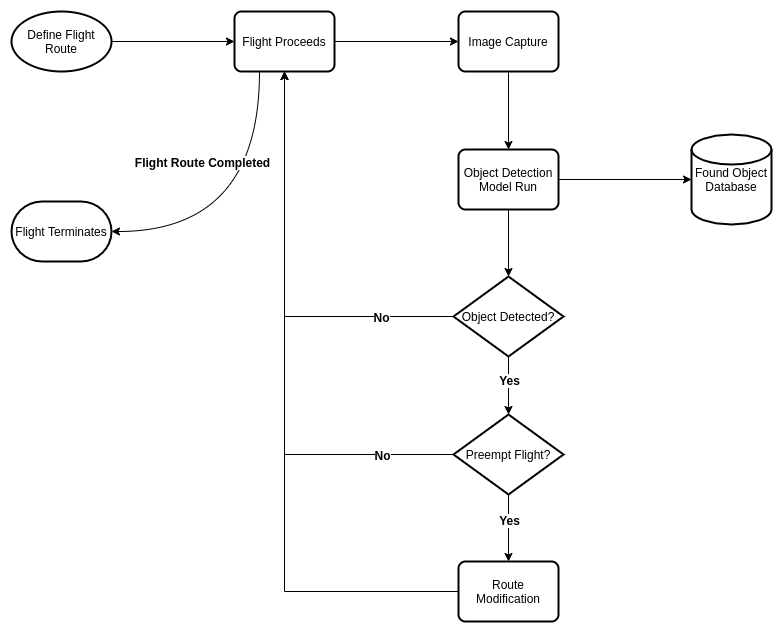
\includegraphics[width=1\linewidth]{assets/activity-diagram.png}
\caption{Activity Diagram}
\label{activity_diagram}
\end{figure}

\chapter{Proposed Solution}
\section{Proposed Solution}
\begin{figure}[h]
\centering
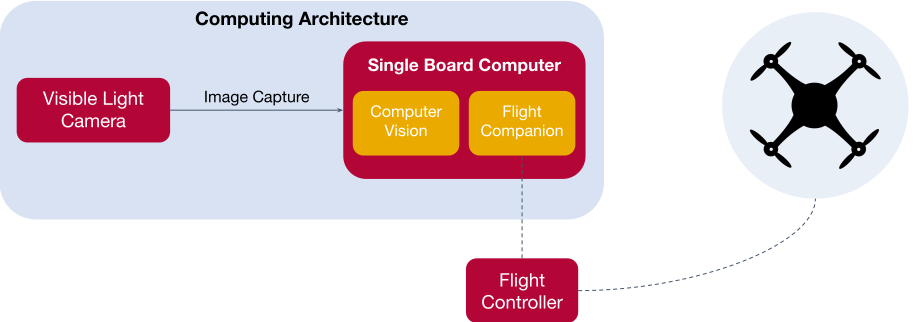
\includegraphics[width=1\linewidth]{assets/proposed-solution.png}
\caption{Proposed Solution}
\label{proposed_solution}
\end{figure}
\subsection{Hardware}
\paragraph{Single Board Computer} Nvidia Jetson Nano - 4 GB

A single board computer was imperative to achieve the non-functional design requirements outlined in~\ref{requirements}, because of their low cost, energy efficiency, size and modularity. After researching performance metrics for single board computers (SBCs) across a variety of indsutry standard computer vision models, it was determined that the NVidia Jetson Nano would be the most cost-effective and performant SBC choice, especially compared to competing platforms. On one hand, the Raspberry Pi series of SBCs would be satisfactory in regard to power usage, but significantly underpowered for computer vision applications. On the other hand, the Google Coral TPU Dev Board boasted incredible inference speeds where comparison was possible, but its major caveat consisted of only being capable of running Tensor Flow Lite (TFLite) models, which would have a significant detriment on the modularity and flexibility of the overall platform.

\paragraph{UAV Frame} HolyBro S500v2 Kit

In order to achieve the requirements of competitive flight time (compared to enterprise solutions), an accessible pricepoint, and a suitable size to mount all components, the choice was quickly narrowed down to a \textit{quadcopter}, meaning a UAV with four propellers. A quadcopter is useful for this use-case because...

\paragraph{Flight Controller} PixHawk 4

The flight controller acts as the textit{brain} of a UAV system. The PixHawk 4 was chosen because it satisfies three primary requirements of this project's design:
\begin{itemize}
\item {Autonomous flight}
\item {Detailed logging}
\item {Interface to companion computer}
\end{itemize}

\subsection{Software}
\paragraph{Flight Software} QGroundControl

QGroundControl boasts a high degree of compatibility with leading consumer and enterprise-level drone systems, including the HolyBro S500 and PixHawk 4 platform we chose for this project.
\begin{itemize}
    \item {Various route-planning tools}
    \item {Universal compatibility}
    \item {Open-souce software}
\end{itemize}

\subsection{Developer Tools}
\paragraph{JetPack Software Development Kit}

Includes:
\begin{itemize}
    \item {Jetson Linux Driver Package (L4T)}
    \item {Ubuntu 18.04 LTS Build}
    \item {CUDA accelerated libraries and APIs}
    \item {Samples, documentation and developer tools}
\end{itemize}

\paragraph{NGC Catalog} Package Manager

Easy access to AI building blocks
\begin{itemize}
    \item {Models}
    \item {Containers}
    \item {SDKs}
\end{itemize}

\chapter{System Evaluation}

\section{System Evaluation}
\subsection{Computer Vision Performance}
% Please add the following required packages to your document preamble:
% \usepackage{multirow}
% \usepackage{graphicx}
\begin{table}[]
\resizebox{\textwidth}{!}{%
\begin{tabular}{|l|l|l|l|l|l|l|l|}
\hline
Model                             & Application                            & Power Profile & Inference Speed & Power Consumption & GPU Latency & GPU Load & CPU Load \\ \hline
\multirow{2}{*}{Inception v4}     & \multirow{6}{*}{Classification}        & 5W            & 10.58 FPS       & 5.029 W           & 94.477 ms   & 56.16\%  & 85.03\%  \\ \cline{3-8} 
                                  &                                        & 10W           & 10.60 FPS       & 5.570 W           & 94.340 ms   & 70.30\%  & 40.31\%  \\ \cline{1-1} \cline{3-8} 
\multirow{2}{*}{VGG-19}           &                                        & 5W            & 10.09 FPS       & 5.150 W           & 99.121 ms   & 58.92\%  & 84.74\%  \\ \cline{3-8} 
                                  &                                        & 10W           & 10.04 FPS       & 5.004 W           & 99.596 ms   & 39.79\%  & 49.45\%  \\ \cline{1-1} \cline{3-8} 
\multirow{2}{*}{ResNet 50}        &                                        & 5W            & 36.67 FPS       & 5.029 W           & 27.268 ms   & 54.56\%  & 86.90\%  \\ \cline{3-8} 
                                  &                                        & 10W           & 36.88 FPS       & 5.564 W           & 27.116 ms   & 63.80\%  & 41.56\%  \\ \hline
\multirow{2}{*}{SSD Mobilenet v1} & \multirow{4}{*}{Object Detection}      & 5W            & 42.56 FPS       & 4.360 W           & 23.498 ms   & 58.49\%  & 94.82\%  \\ \cline{3-8} 
                                  &                                        & 10W           & 42.64 FPS       & 5.097 W           & 23.454 ms   & 77.88\%  & 44.77\%  \\ \cline{1-1} \cline{3-8} 
\multirow{2}{*}{TinyYolo v3}      &                                        & 5W            & 47.65 FPS       & 3.541 W           & 20.987 ms   & 14.25\%  & 95.31\%  \\ \cline{3-8} 
                                  &                                        & 10W           & 47.60 FPS       & 4.325 W           & 21.008 ms   & 24.64\%  & 50.62\%  \\ \hline
\multirow{2}{*}{UNet}             & \multirow{2}{*}{Semantic Segmentation} & 5W            & 16.59 FPS       & 3.281 W           & 60.266 ms   & 0.45\%   & 92.68\%  \\ \cline{3-8} 
                                  &                                        & 10W           & 16.62 FPS       & 5.882 W           & 60.177 ms   & 89.76\%  & 36.53\%  \\ \hline
\multirow{2}{*}{Super Resolution} & \multirow{2}{*}{Image Processing}      & 5W            & 15.26 FPS       & 6.396 W           & 65.524 ms   & 86.82\%  & 78.00\%  \\ \cline{3-8} 
                                  &                                        & 10W           & 15.26 FPS       & 5.943 W           & 65.547 ms   & 82.51\%  & 36.94\%  \\ \hline
\multirow{2}{*}{OpenPose}         & \multirow{2}{*}{Pose Estimation}       & 5W            & 14.64 FPS       & 3.258 W           & 68.313 ms   & 0.26\%   & 92.46\%  \\ \cline{3-8} 
                                  &                                        & 10W           & 14.64 FPS       & 3.968 W           & 68.320 ms   & 0.00\%   & 46.42\%  \\ \hline
\end{tabular}%
}
\end{table}

\subsection{Price}
% Please add the following required packages to your document preamble:
% \usepackage{graphicx}
\begin{table}[]
% \resizebox{\textwidth}{!}{%
\begin{tabular}{|l|l|}
\hline
\textbf{Product}           & \textbf{Price} \\ \hline
NVIDIA Jetson Nano 4 GB    & \$120          \\ \hline
HolyBro S500 v2 Kit        & \$355          \\ \hline
Pixhawk 4                  & \$70           \\ \hline
8000mAh Battery \& Charger & \$270          \\ \hline
IMX219-77 Camera           & \$20           \\ \hline
\textbf{Total}             & \textbf{\$835} \\ \hline
\end{tabular}%
% }
\end{table}

\subsection{Comparison}
% Please add the following required packages to your document preamble:
% \usepackage{graphicx}
\begin{table}[]
\resizebox{\textwidth}{!}{%
\begin{tabular}{l|l|l|}
\cline{2-3}
                                                 & \textbf{Prototype}                & \textbf{Industry Standard Averages} \\ \hline
\multicolumn{1}{|l|}{\textbf{Flight Time}}       & 25.7 min                          & 31.5 min                            \\ \hline
\multicolumn{1}{|l|}{\textbf{Computer Vision}}   & Real-time up to $\sim$480p 45 fps & No                                  \\ \hline
\multicolumn{1}{|l|}{\textbf{Autonomous Flight}} & Yes                               & Yes                                 \\ \hline
\multicolumn{1}{|l|}{\textbf{Modularity}}        & High                              & Minimal                             \\ \hline
\multicolumn{1}{|l|}{\textbf{Price}}             & \$835                             & \$6,750                             \\ \hline
\end{tabular}%
}
\end{table}


\backmatter
% \bibliography{bibliography}
\end{document}
